\documentclass[]{beamer}
\usetheme{KUL}
\usepackage{multirow}
\usepackage{multicol}
\usepackage{tikz}
\usepackage{ulem}
\usepackage{siunitx}
\newcommand\itemS{\item[\textbf{\S}]}
\definecolor{darkgreen}{rgb}{0,0.598,0.199}
\usepackage{times} % set font on times new roman
\usepackage{eurosym} % package for Euro sign
\usepackage{lineno}   % package for line numbering
\usepackage{hyperref} % this is for url links
\usepackage{subcaption}  % this package enables one to put several figures next to each other
\usepackage{textcomp}
\usepackage{setspace}
\usepackage{gensymb}

%----------------------------------
% Fill in the essential Information
%----------------------------------

\title[The Variability of the Belgian Business Survey Indicator]{The Variability of the Belgian Business Survey Indicator}
\subtitle{Analysis and Predictive Power}
\author[F.\ Van Boeckel]{Fabrice VAN BOECKEL} % between [] is short name, between {} is long name
\date{\today} % Here you can also just type something, e.g. October 10, 2017
\institute[KU Leuven]{Faculty of Science\\ Department of Mathematics\\ Leuven Statistics Research Centre}

%----------------------------------
% ACTUAL PRESENTATION STARTS HERE
%----------------------------------


\begin{document}

% TITEL PAGE	
	{
		\setbeamertemplate{headline}{} %define local, empty header for title page
		\setbeamertemplate{footline}{} %define local, empty footer for title page
		\maketitle
	}
	\addtocounter{framenumber}{-1} % We don't count the title page

% FRAME 1 
\section{Introduction}
\begin{frame}{Frame 1}
\begin{itemize}
    \item some text
    
\end{itemize}
\begin{kulblock}{Landslide}
    A landslide is the downhill movement of soil mass
\end{kulblock}
\end{frame}

% FRAME 2
\begin{frame}{A figure}
\centering
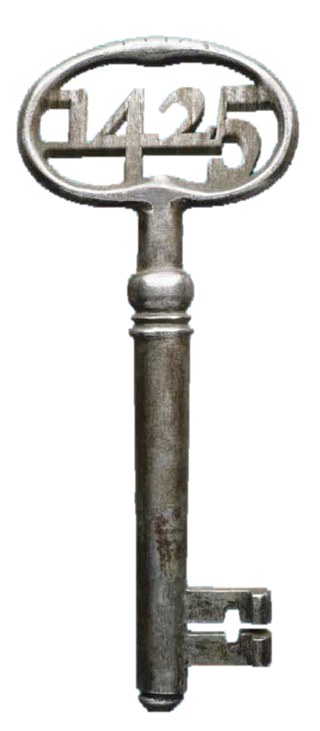
\includegraphics[width=2cm]{Images/sleutel.png}
\end{frame}

% FRAME 3
\begin{frame}{A table}
\centering
\begin{tabular}{|c|c|}
    \hline
     \bf X & \bf Y \\ \hline
     x & y \\ \hline 
\end{tabular}
\end{frame}

\end{document}